\documentclass{standalone}
\usepackage{tikz}
\begin{document}
    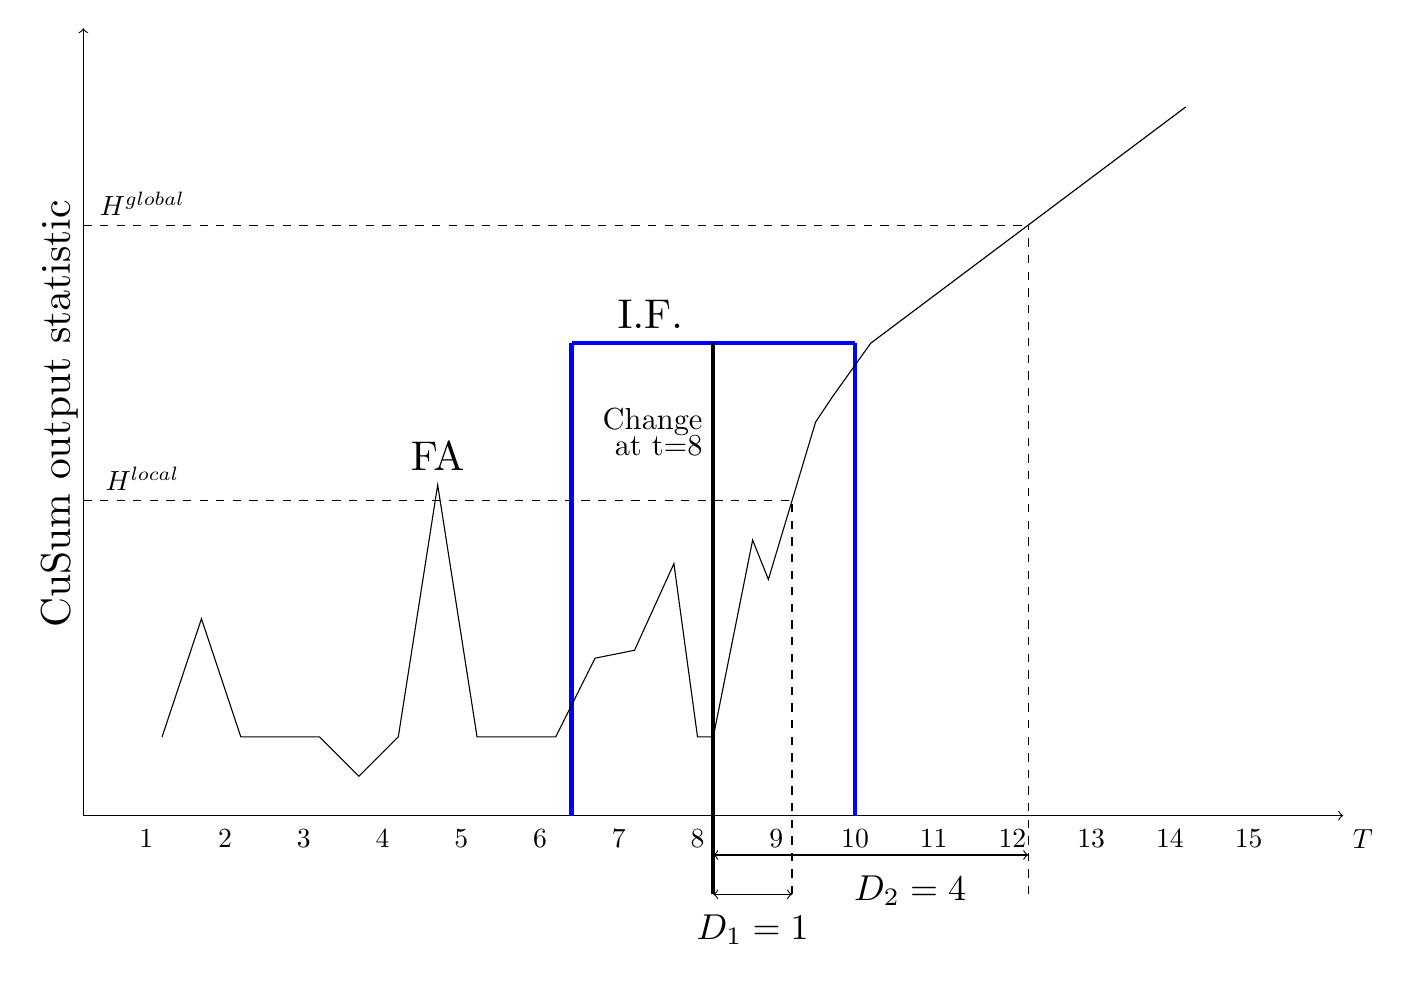
\begin{tikzpicture}[scale=1.0, xscale=1]
%    \def\ticksz{0.2};
    \def\rad{0.15};
    \def\w{1.8};
    \def\h{6};
    
    \draw [->] (0,0) -- (16,0) node [below right] at (16.0,-0.05) {$T$};
    \draw [->] (0,0) -- (0,10) node[rotate=90, scale=1.5] [left] at (-0.3, 8) {CuSum output statistic};
%%%%%%%%%%%%%%%%%%%%%%%%%%%
%% Circles for reference
%    \foreach \x in {1,...,7}
%    {
%        %\draw[fill=white] (\x, 1) circle (\rad); 
%        \node[below] at (\x, -1.5) {\x};
%    }
%    \foreach \x in {8,...,15}
%    {
%        %\draw[fill=white] (\x, \x-7) circle (\rad); 
%        \node[below] at (\x, -1.5) {\x};
%    }
    
    \foreach \x in {1,...,15}
        \node[below] at (\x-0.2, -0.05) {\x};
    % indicator function
    \draw[blue, line width=0.55mm] (8-\w, 0) -- (8-\w,\h);
    \draw[blue, line width=0.5mm] (8+\w, 0) -- (8+\w,\h);
    \draw[blue, line width=0.5mm] (8-\w,\h) -- (8+\w,\h);
    \node[above, scale=1.5] at (8-0.8, \h) {I.F.};
    % output stat
    \draw (1,1)--(1.5, 1+1.5) -- (2,1) -- (3,1) -- (3.5, 1-0.5) -- (4,1) -- (4.5,3+1.2) -- (5,1) -- (6,1) -- (6.5,2.0) -- (7,2.1) -- (7.5, 3.2) -- (7.8, 1) -- (8,1) -- (8.5, 3.5) -- (8.7, 3.0) -- (9, 4)--(9.3, 5) -- (9.5, 5.3) -- (10, 6) -- (12, 7.5) -- (14, 9);
    
    % FA
    \node[above, scale=1.5] at (4.5, 3+1.2) {FA};
    % global optimum
    \draw[dashed] (0, 7.5) -- (12, 7.5);
    \draw[dashed] (12, 0-1) -- (12, 7.5);
    % global optim param
    \node[above] at (0+0.75, 7.5) {$H^{global}$};
    % local optimum
    \draw[dashed] (0, 4) -- (9, 4);
    \draw[dashed] (9, 0-1) -- (9, 4);
    % local optim param
    \node[above] at (0+0.75, 4) {$H^{local}$};
    % changepoint
    \draw[line width=0.5mm] (8,0-1) -- (8, \h);
    \node[left, scale=1.1] at (8, \h-1) {Change};
    \node[left, scale=1.1] at (8, \h-1.3) {at t=8};
    % delay 1
    \draw[<->] (8,0-1) -- (9, 0-1);
    \node[below, scale=1.3] at (8.5, -1.1) {$D_1=1$};
    % delay 2
    \draw[<->] (8, 0-0.5) -- (12, 0-0.5);
    \node[below, scale=1.3] at (10.5, -0.6) {$D_2=4$};
    \end{tikzpicture}
\end{document}
